%experimental.tex
%\section{Experimental Evaluation}\label{sec.experimental}



\subsection{Experimental Evaluation of Two-Step Method}
\label{chUV_AMBC.sec.twoStepExp}

In this Section we report an experimental evaluation of the two-step
algorithm reported in Section \ref{chUV_AMBC.sec.twoStepMethod}.

The first step is identifying the gravitational and buoyancy
parameters for the \ac{UV} using the adaptive tracking controller for
plant model (\ref{chUV_AMBC.eq.plantQS}).  The reference trajectory
was constant in translational position and heading, with slow changes
in pitch and roll to provide quasi-static motion.  For this experiment
we used a sinusoidal pitch reference trajectory with a magnitude of
$0.2$ rad and frequency of $34$ Hz and a sinusoidal roll reference
trajectory with a magnitude of $0.15$ rad and frequency of $42$
Hz. The gains used were $k_p=300$, $k_d=100$,
$\gamma_{g}=\gamma_{b_1}=\gamma_{b_2}=0.5$, and $\gamma_{b_3}=10.0$.
Over a 90 minute experiment the gravitational and buoyancy parameters
were stable and converged to the physically realistic values shown in
Table \ref{chUV_AMBC.tb.quasistatic}.

\begin{table}[htbp]
\ssp
\caption{Gravitational Parameters Identified During Quasi-Static Motion}
\begin{center}
\begin{tabular}{c|cccc}
 & $g$ & $b_1$ & $b_2$ & $b_3$ \\
 & {\it N} & {\it N m} & {\it N m} & {\it N m} \\ \hline
Final & 3.59 & 1.696 & 3.09 & 300 \\
\end{tabular}
\end{center}
\label{chUV_AMBC.tb.quasistatic}
\vspace*{-5mm}
\end{table}


The second step uses the identified parameters from Table
\ref{chUV_AMBC.tb.quasistatic} in a \ac{AMBC} which estimates the
mass and drag parameters, as described in Section
\ref{chUV_AMBC.sec.twoStepMethod}.
%
In the second step of the two-step \ac{AMBC} algorithm the reference
trajectory specified was RefTraj1 from Table
\ref{chUV_AMBC.tb.expStat}; the mass and drag parameters were
initialized to zero; and the gains used were $k_p=300$, $k_d=1000$,
$\gamma_{m_i}=1000$, and $\gamma_{d_i}=5000$.  Over a four and a half
hour experiment all 12 mass and drag parameters were observed to be
stable and converge to physically realistic values.  Table
\ref{chUV_AMBC.tb.dynParam} records the initial and final states for
each dynamic parameter estimate.

\begin{table}[htbp]
\ssp
\caption{Parameters Identified with two-step \ac{AMBC} during 
  Dynamic Motion Trajectory-Tracking}
\begin{center}
\begin{tabular}{c|cccc}
 & $m_i(t_o)$ & $m_i(t_f)$ & $d_i(t_o)$ & $d_i(t_f)$ \\ \hline
Trans X \ac{DOF} & 0.0 {\it kg}& 628 {\it kg}& 0.0 {\it $\frac{\text{N}~\text{s}^2}{\text{m}^2}$}& -1259 {\it $\frac{\text{N}~\text{s}^2}{\text{m}^2}$}\\
Trans Y \ac{DOF} & 0.0 {\it kg}& 791 {\it kg}& 0.0 {\it $\frac{\text{N}~\text{s}^2}{\text{m}^2}$}& -1429 {\it $\frac{\text{N}~\text{s}^2}{\text{m}^2}$}\\
Trans Z \ac{DOF} & 0.0 {\it kg}&1043 {\it kg}& 0.0 {\it $\frac{\text{N}~\text{s}^2}{\text{m}^2}$}& -3083 {\it $\frac{\text{N}~\text{s}^2}{\text{m}^2}$}\\
Angular X \ac{DOF} & 0.0 {\it kg $\text{m}^2$}& 95.7 {\it kg $\text{m}^2$}& 0.0 {\it N $\text{s}^2$}& -727.1 {\it N $\text{s}^2$}\\
Angular Y \ac{DOF} & 0.0 {\it kg $\text{m}^2$}& 145.3 {\it kg $\text{m}^2$}& 0.0 {\it N $\text{s}^2$}& -783.4 {\it N $\text{s}^2$}\\
Angular Z \ac{DOF} & 0.0 {\it kg $\text{m}^2$}& 110.2 {\it kg $\text{m}^2$}& 0.0 {\it N $\text{s}^2$}& -465.6 {\it N $\text{s}^2$}\\
\end{tabular}
\end{center}
\label{chUV_AMBC.tb.dynParam}
\vspace*{-5mm}
\end{table}

\subsubsection{Two-Step \ac{AMBC} Trajectory Tracking Performance}

Figure \ref{chUV_AMBC.fig.MNE_All} compares the performance of the
second step of the two-step \ac{AMBC} to a \ac{PDC} with comparable
gains.  These two plots contain the exponential position and velocity
\ac{MNE} for the \ac{PDC} and two-step \ac{AMBC} experimental run.
Both controllers were following the reference trajectory RefTraj1 from
Table \ref{chUV_AMBC.tb.expStat} as well as using $k_p=300$ and
$k_d=100$.
%
The \ac{PDC} \acp{MNE} values were calculated using 10 minutes of
data.  
%
The two-step \ac{AMBC} \acp{MNE} values were calculated
for consecutive 15 minutes windows.
%
Note that after parameter convergence the two-step \ac{AMBC} provides
$30\%$ better position tracking and $8\%$ worse velocity tracking than
\ac{PDC} with similar gains.
%
% Thus two-step \ac{AMBC} Since position trajectory tracking is typically
% the goal of current \ac{UV} controllers, this controller provides
% significant advantages over standard \ac{PDC} control method for 6-\ac{DOF}
% motion.

Table \ref{chUV_AMBC.tb.trajTrackMAE} reports the trajectory tracking
\ac{MAE} values of individual \ac{DOF} for both the \ac{PDC} and
two-step \ac{AMBC} experiments.
%
The \ac{PDC} \acp{MAE} values were calculated using 10 minutes of
data.  
%
The two-step \ac{AMBC} \acp{MAE} values were calculated
for consecutive 15 minutes windows.
%
For each of the position \ac{DOF}, two-step \ac{AMBC} \ac{MAE} values
were smaller than \ac{PDC} values.
%
With the exception of heading, two-step \ac{AMBC} position trajectory
tracking improved in each \ac{DOF} as the parameter adaptation process
progressed.
%
Of the velocity \ac{DOF}, two-step \ac{AMBC} only outperformed
\ac{PDC} in the x and y angular velocity \ac{DOF}.
%
With the exception of y angular velocity, two-step \ac{AMBC} velocity
trajectory-tracking performance degraded slightly as the parameter
adaptation process occurred.
%
For the \ac{DOF} in which trajectory-tracking is not improving, this
could be an effect of unmodeled thruster dynamics or other dynamics
which are not included in the uncoupled lumped-parameter model of
\ac{UV} dynamics used in our \ac{AMBC} algorithm.
%
However, taken as a whole, this experimental evaluation indicates that
\ac{AMBC} can provide increased trajectory-tracking performance in the
presence of unmodeled thruster dynamics.




\begin{center}
\begin{figure}[htbp]
  \begin{center}
    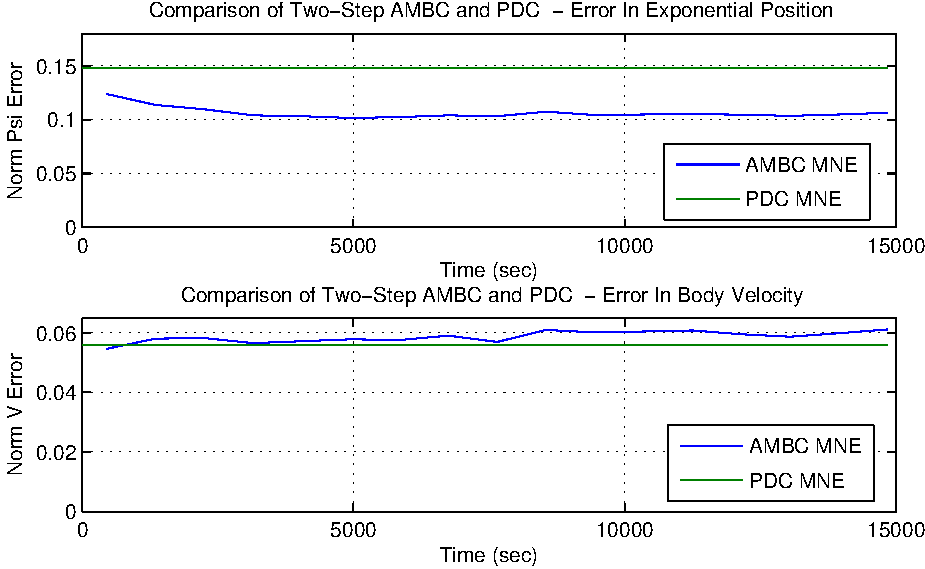
\includegraphics[width=150mm]{./chUV_AMBC/images/MNE_All}
  \end{center}
  \caption{ Exponential position and velocity \ac{MNE} values for the
    experimental evaluations of two controllers, \ac{PDC} and two-step
    \ac{AMBC}.  Both controllers were following the same reference
    trajectory (RefTraj1 from Table \ref{chUV_AMBC.tb.expStat}) as
    well as using the gains $k_p=300$ and $k_d=100$.  The \ac{PDC}
    \ac{MNE} values were calculated using 10 minutes of data, this
    single value is plotted in green across the entire figure.  The
    two-step \ac{AMBC} \ac{MNE} values were calculated for consecutive
    15 minute windows and plotted in blue. }
  \label{chUV_AMBC.fig.MNE_All}
\vspace*{-5mm}
\end{figure}
\end{center}

% \begin{sidewaystable*}
% \ssp
% \fontsize{8pt}{8pt}\selectfont
% \caption{Mean Absolute Error values over different pieces on time.}
% \begin{center}
% \begin{tabular}{c|ccccccccccccc} 
%     Parameter & Time  &&&&&&&&&&&& \\              
%           Set & Block & PosX & PosY & PosZ & Hea & Pit & Rol & BodVelX & BodVelY & BodVelZ & AngVelX & AngVelY & AngVelZ \\ \hline 
% \\
% \ac{PDC} Exp  &      ALL   & 0.076m & 0.061m & 0.058m & 0.028rad & 0.047rad & 0.04rad & 0.0172m/s & 0.021m/s & 0.0156m/s & 0.021rad/s & 0.028rad/s & 0.0078rad/s \\ \hline
% \\
% \ac{AMBC} Exp & 0-14 min & 0.059m & 0.051m & 0.064m & 0.021rad & 0.023rad & 0.0181rad & 0.022m/s & 0.023m/s & 0.0194m/s & 0.0136rad/s & 0.017rad/s & 0.0134rad/s \\
% \\
% \ac{AMBC} Exp & 0-14 min & 0.051m & 0.045m & 0.063m & 0.022rad & 0.0196rad & 0.0184rad & 0.024m/s & 0.023m/s & 0.02m/s & 0.0137rad/s & 0.0157rad/s & 0.0162rad/s \\
% \\
% \ac{AMBC} Exp & 15-29 min & 0.047m & 0.046m & 0.057m & 0.021rad & 0.0196rad & 0.0171rad & 0.023m/s & 0.025m/s & 0.02m/s & 0.013rad/s & 0.0169rad/s & 0.0153rad/s \\
% \\
% \ac{AMBC} Exp & 30-44 min & 0.046m & 0.045m & 0.054m & 0.0192rad & 0.018rad & 0.0165rad & 0.023m/s & 0.025m/s & 0.0196m/s & 0.0136rad/s & 0.0157rad/s & 0.0149rad/s \\
% \\
% \ac{AMBC} Exp & 45-59 min & 0.046m & 0.043m & 0.052m & 0.021rad & 0.0174rad & 0.0162rad & 0.024m/s & 0.025m/s & 0.019m/s & 0.0136rad/s & 0.0162rad/s & 0.0161rad/s \\
% \\
% \ac{AMBC} Exp & 60-74 min & 0.047m & 0.047m & 0.046m & 0.0198rad & 0.0174rad & 0.0156rad & 0.023m/s & 0.027m/s & 0.0179m/s & 0.0138rad/s & 0.0168rad/s & 0.0152rad/s \\
% \\
% \ac{AMBC} Exp & 75-89 min & 0.047m & 0.045m & 0.05m & 0.021rad & 0.0168rad & 0.0155rad & 0.024m/s & 0.024m/s & 0.0192m/s & 0.0143rad/s & 0.0164rad/s & 0.0155rad/s \\
% \\
% \ac{AMBC} Exp & 90-104 min & 0.046m & 0.046m & 0.052m & 0.022rad & 0.0174rad & 0.0155rad & 0.024m/s & 0.026m/s & 0.0198m/s & 0.014rad/s & 0.0165rad/s & 0.0162rad/s \\
% \\
% \ac{AMBC} Exp & 105-119 min & 0.048m & 0.044m & 0.05m & 0.022rad & 0.0162rad & 0.0153rad & 0.021m/s & 0.025m/s & 0.021m/s & 0.0133rad/s & 0.0159rad/s & 0.0151rad/s \\
% \\
% \ac{AMBC} Exp & 120-134 min & 0.049m & 0.048m & 0.054m & 0.021rad & 0.0182rad & 0.015rad & 0.023m/s & 0.027m/s & 0.023m/s & 0.0145rad/s & 0.0169rad/s & 0.016rad/s \\
% \\
% \ac{AMBC} Exp & 135-149 min & 0.049m & 0.045m & 0.05m & 0.022rad & 0.0177rad & 0.0145rad & 0.025m/s & 0.026m/s & 0.021m/s & 0.0145rad/s & 0.0172rad/s & 0.0165rad/s \\
% \\
% \ac{AMBC} Exp & 150-164 min & 0.05m & 0.046m & 0.049m & 0.021rad & 0.0166rad & 0.0155rad & 0.024m/s & 0.026m/s & 0.021m/s & 0.0143rad/s & 0.0161rad/s & 0.0167rad/s \\
% \\
% \ac{AMBC} Exp & 165-179 min & 0.049m & 0.046m & 0.052m & 0.021rad & 0.0168rad & 0.0151rad & 0.024m/s & 0.026m/s & 0.022m/s & 0.0145rad/s & 0.0167rad/s & 0.0153rad/s \\
% \\
% \ac{AMBC} Exp & 180-194 min & 0.048m & 0.047m & 0.05m & 0.021rad & 0.017rad & 0.0149rad & 0.024m/s & 0.024m/s & 0.021m/s & 0.0141rad/s & 0.0165rad/s & 0.016rad/s \\
% \\
% \ac{AMBC} Exp & 195-209 min & 0.05m & 0.045m & 0.049m & 0.022rad & 0.0169rad & 0.0149rad & 0.023m/s & 0.026m/s & 0.02m/s & 0.0139rad/s & 0.0163rad/s & 0.0161rad/s \\
% \\
% \ac{AMBC} Exp & 210-224 min & 0.05m & 0.046m & 0.049m & 0.021rad & 0.0174rad & 0.0147rad & 0.024m/s & 0.027m/s & 0.021m/s & 0.0142rad/s & 0.0166rad/s & 0.0148rad/s \\
% \\
% \ac{AMBC} Exp & 225-239 min & 0.047m & 0.046m & 0.054m & 0.022rad & 0.0172rad & 0.0147rad & 0.025m/s & 0.026m/s & 0.023m/s & 0.0145rad/s & 0.0164rad/s & 0.0169rad/s \\
% \end{tabular}
% \end{center}
% \label{chUV_AMBC.tb.MAE}
% \end{sidewaystable*}


\begin{sidewaystable*}
\ssp
\fontsize{10pt}{10pt}\selectfont
\caption{\acf{MAE} values for both the \ac{PDC} and two-step \ac{AMBC}
  experiments.  The \ac{MAE} for each \ac{DOF} is shown. 10 minutes of
  experimental data were used to calculate the \ac{PDC} \acp{MAE}.
  \ac{AMBC} \acp{MAE} were calculated for consecutive 15 minute
  windows spread over the 3 hour experiment.}
\begin{center}
\begin{tabular}{c|ccccccccccccc} 
    Parameter & Time  &&&&&&&&&&&& \\              
          Set & Block & PosX & PosY & PosZ & Hea & Pit & Rol & BodVelX & BodVelY & BodVelZ & AngVelX & AngVelY & AngVelZ \\  
      {\it -} & {\it min} & {\it m}   &  {\it m}  &  {\it m}  &{\it rad} &{\it rad} &{\it rad} &{\it m/sec} &{\it m/sec} &{\it m/sec} &{\it rad/sec} &{\it rad/sec} &{\it rad/sec} \\ \hline 
\\
\ac{PDC} Exp  &    -   & 0.076  & 0.061  & 0.058  & 0.028  & 0.047  & 0.04  & 0.0172  & 0.021  & 0.0156  & 0.021  & 0.028  & 0.0078  \\ \hline
\\
\ac{AMBC} Exp & 0-14   & 0.059  & 0.051  & 0.064  & 0.021  & 0.023  & 0.0181  & 0.022  & 0.023  & 0.0194  & 0.0136  & 0.017  & 0.0134  \\
\\
\ac{AMBC} Exp & 15-29   & 0.051  & 0.045  & 0.063  & 0.022  & 0.0196  & 0.0184  & 0.024  & 0.023  & 0.02  & 0.0137  & 0.0157  & 0.0162  \\
\\
\ac{AMBC} Exp & 30-44   & 0.047  & 0.046  & 0.057  & 0.021  & 0.0196  & 0.0171  & 0.023  & 0.025  & 0.02  & 0.013  & 0.0169  & 0.0153  \\
\\
\ac{AMBC} Exp & 45-59   & 0.046  & 0.045  & 0.054  & 0.0192  & 0.018  & 0.0165  & 0.023  & 0.025  & 0.0196  & 0.0136  & 0.0157  & 0.0149  \\
\\
\ac{AMBC} Exp & 60-74   & 0.046  & 0.043  & 0.052  & 0.021  & 0.0174  & 0.0162  & 0.024  & 0.025  & 0.019  & 0.0136  & 0.0162  & 0.0161  \\
\\
\ac{AMBC} Exp & 75-89   & 0.047  & 0.047  & 0.046  & 0.0198  & 0.0174  & 0.0156  & 0.023  & 0.027  & 0.0179  & 0.0138  & 0.0168  & 0.0152  \\
\\
\ac{AMBC} Exp & 90-104   & 0.047  & 0.045  & 0.05  & 0.021  & 0.0168  & 0.0155  & 0.024  & 0.024  & 0.0192  & 0.0143  & 0.0164  & 0.0155  \\
\\
\ac{AMBC} Exp & 105-119   & 0.046  & 0.046  & 0.052  & 0.022  & 0.0174  & 0.0155  & 0.024  & 0.026  & 0.0198  & 0.014  & 0.0165  & 0.0162  \\
\\
\ac{AMBC} Exp & 120-134  & 0.048  & 0.044  & 0.05  & 0.022  & 0.0162  & 0.0153  & 0.021  & 0.025  & 0.021  & 0.0133  & 0.0159  & 0.0151  \\
\\
\ac{AMBC} Exp & 135-149   & 0.049  & 0.048  & 0.054  & 0.021  & 0.0182  & 0.015  & 0.023  & 0.027  & 0.023  & 0.0145  & 0.0169  & 0.016  \\
\\
\ac{AMBC} Exp & 150-164   & 0.049  & 0.045  & 0.05  & 0.022  & 0.0177  & 0.0145  & 0.025  & 0.026  & 0.021  & 0.0145  & 0.0172  & 0.0165  \\
\\
\ac{AMBC} Exp & 165-179   & 0.05  & 0.046  & 0.049  & 0.021  & 0.0166  & 0.0155  & 0.024  & 0.026  & 0.021  & 0.0143  & 0.0161  & 0.0167  \\
\\
\ac{AMBC} Exp & 180-194   & 0.049  & 0.046  & 0.052  & 0.021  & 0.0168  & 0.0151  & 0.024  & 0.026  & 0.022  & 0.0145  & 0.0167  & 0.0153  \\
\\
\ac{AMBC} Exp & 195-209   & 0.048  & 0.047  & 0.05  & 0.021  & 0.017  & 0.0149  & 0.024  & 0.024  & 0.021  & 0.0141  & 0.0165  & 0.016  \\
\\
\ac{AMBC} Exp & 210-224   & 0.05  & 0.045  & 0.049  & 0.022  & 0.0169  & 0.0149  & 0.023  & 0.026  & 0.02  & 0.0139  & 0.0163  & 0.0161  \\
\\
\ac{AMBC} Exp & 225-239   & 0.05  & 0.046  & 0.049  & 0.021  & 0.0174  & 0.0147  & 0.024  & 0.027  & 0.021  & 0.0142  & 0.0166  & 0.0148  \\
\\
\ac{AMBC} Exp & 240-255   & 0.047  & 0.046  & 0.054  & 0.022  & 0.0172  & 0.0147  & 0.025  & 0.026  & 0.023  & 0.0145  & 0.0164  & 0.0169  \\
\end{tabular}
\end{center}
\label{chUV_AMBC.tb.trajTrackMAE}
\end{sidewaystable*}


\subsubsection{Two-Step \ac{AMBC} Parameter Cross-Validation}

In addition to providing trajectory-tracking, \ac{AMBC} has also been
proposed to identify \ac{UV} models.
%
Two questions arise: 
%
\begin{itemize}
\item ``How good is the identified model at reproducing vehicle performance?''
%``When considering the time series of parameter
%estimations, will the capacity of the models which used these
%parameter estimations get better at matching vehicle performance as
%time increases?''
%
\item``Considering the time series of parameter estimates, do the
  resulting plant models get better at matching \ac{JHUROV}
  performance as the parameter adaptation process progresses?''
\end{itemize}
%

To address these questions we preformed a cross-validation experiment
(Appendix \ref{appenJHUHTF.sec.paramEvalMethod}) by driving the
\ac{JHUROV} to follow RefTraj2 from Table \ref{chUV_AMBC.tb.expStat}.
%the \ac{UV} states and thrust inputs were recorded for 10 minutes.
%
\Cref{chUV_AMBC.fig.posOLO,chUV_AMBC.fig.angVelOLO,chUV_AMBC.fig.bodVelOLO}
show the ability of the identified model to match vehicle performance
in forward simulation increases during parameter adaptation.
%
Each Figure shows experimentally measured states verses the states
from numerical simulations; each numerical simulation uses a model
identified by the two-step \ac{AMBC} after a set amount of time.
%
Each \ac{JHUROV} simulation used the thrust inputs recorded and
initial \ac{JHUROV} states to create a forward
simulation. % of vehicle performance.
%
All eight open-loop-stable states are plotted.
%
In both the plots and listed \ac{MAE} values, the capacity of the
identified parameters to model vehicle performance in every \ac{DOF}
increases as time progresses.
%
The fact that the parameter estimates are progressively improving
suggests that the parameter adaptation process is working despite the
presence of unmodeled thruster dynamics.



As was seen with \ac{AID} and \ac{LS} in Sections
\ref{chUV_AID.sec.UVSO3exp} and \ref{chUV_AID.sec.UVSE3exp}, the
models identified using two-step \ac{AMBC} were not able to reproduce
the highest frequency fluctuation's observed experimentally (such as
those seen in the x angular velocity subplots of Figure
\ref{chUV_AMBC.fig.angVelOLO}).
%
However, the states shown from simulating a model using the ``5000
sec'' parameter set (the final parameter set included in this
analysis) indicate that \ac{AMBC} can produce parameter estimates
which result in accurate plant models.




\begin{center}
\begin{figure}[htbp]
  \begin{center}
    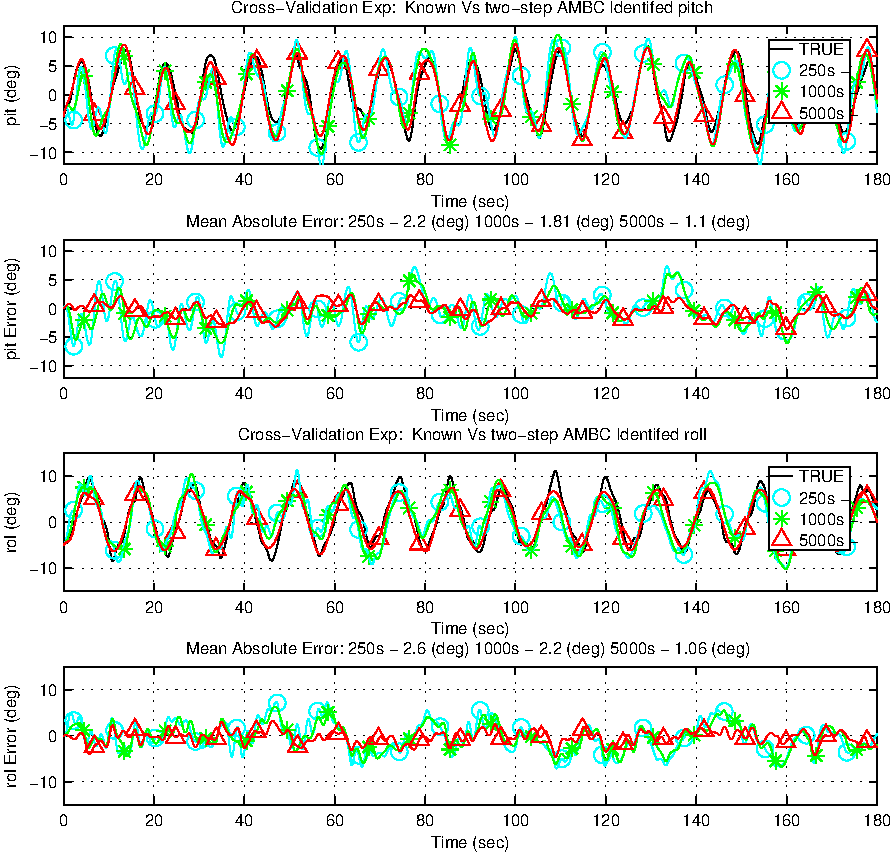
\includegraphics[width=150mm]{./chUV_AMBC/images/OLO_angPos}
  \end{center}
  \caption{ Representative data of experimental and simulated
    \ac{JHUROV} states during 6-\ac{DOF} dynamic operation.  In the
    roll and pitch plots the measured state is plotted together with
    the position estimates from three \ac{JHUROV} simulations. The
    three parameter sets were taken from the time history of parameter
    adaptation recorded during the two-step \ac{AMBC} experiment.  The
    '250s' forward simulation (plotted in blue and marked with
    circles) models \ac{JHUROV} performance using parameters
    identified after 250 seconds of parameter adaptation.  Similarly
    the '1000s' forward simulation (plotted in green and marked with
    stars) and '5000s' forward simulation (plotted in red and marked
    with triangles) use parameters identified after 1000 and 5000
    seconds of parameter adaptation respectively.  For each \ac{DOF},
    the error between the measured positions and their estimates is
    shown.  }
  \label{chUV_AMBC.fig.posOLO}
\end{figure}
\end{center}

\begin{center}
\begin{figure}[htbp]
  \begin{center}
    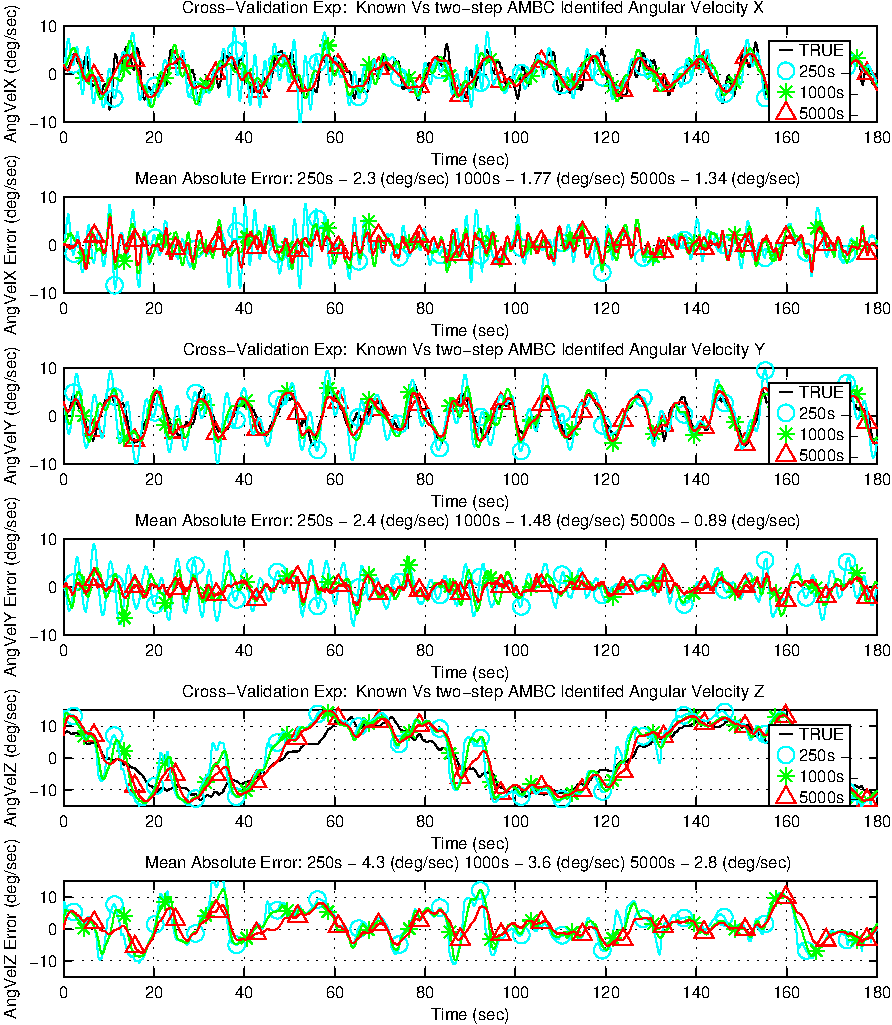
\includegraphics[width=150mm]{./chUV_AMBC/images/OLO_angVel}
  \end{center}
  \caption{ Representative data of experimental and simulated
    \ac{JHUROV} states during 6-\ac{DOF} dynamic operation.  In the
    three angular velocity plots, the measured state is plotted
    together with the velocity estimates from three \ac{JHUROV}
    simulations. The three parameter sets were taken from the time
    history of parameter adaptation recorded during the two-step
    \ac{AMBC} experiment.  See Figure \ref{chUV_AMBC.fig.posOLO}
    caption for further information on each parameter set.  For each
    \ac{DOF}, the error between the measured positions and their
    estimates is shown.  }
  \label{chUV_AMBC.fig.angVelOLO}
\end{figure}
\end{center}

\begin{center}
\begin{figure}[htbp]
  \begin{center}
    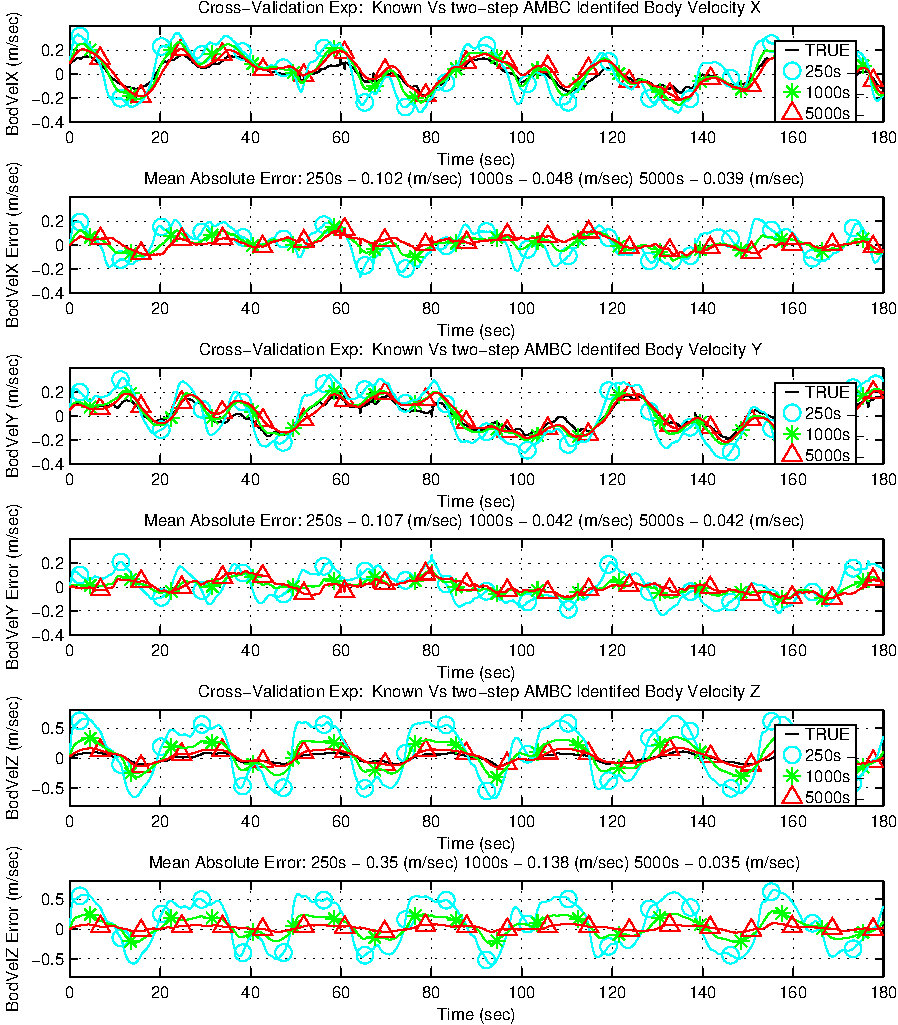
\includegraphics[width=150mm]{./chUV_AMBC/images/OLO_bodyVel}
  \end{center}
  \caption{ Representative data of experimental and simulated
    \ac{JHUROV} states during 6-\ac{DOF} dynamic operation.  In the
    three body velocity plots, the measured state is plotted together
    with the velocity estimates from three \ac{JHUROV}
    simulations. The three parameter sets were taken from the time
    history of parameter adaptation recorded during the two-step
    \ac{AMBC} experiment.  See Figure \ref{chUV_AMBC.fig.posOLO}
    caption for further information on each parameter set.  For each
    \ac{DOF}, the error between the measured positions and their
    estimates is shown.  }
  \label{chUV_AMBC.fig.bodVelOLO}
\end{figure}
\end{center}
 

